%%%%%%%%%%%%%%%%%%%%%%%%%%%%%%%%%%%%%%%%%%%%%%
% Header
\documentclass[11pt]{report}
\usepackage[english]{babel}
\usepackage[utf8x]{inputenc}
\PassOptionsToPackage{hyphens}{url}\usepackage{hyperref}
\usepackage{graphicx}
\usepackage{fullpage}
\usepackage{nicefrac}
\usepackage[lastexercise]{exercise}
\usepackage[dvipsnames]{xcolor}
\usepackage{listings}

\setlength{\parindent}{0cm}

\renewcommand{\ExerciseHeader}{\large\textbf{\ExerciseName~\ExerciseHeaderNB} - \textbf{\ExerciseTitle}\medskip}

\renewcommand{\ExePartHeader}{\medskip\textbf{\ExePartName\ExePartHeaderNB\ExePartHeaderTitle\medskip}}

\begin{document}
%%%%%%%%%%%%%%%%%%%%%%%%%%%%%%%%%%%%%%%%%%%%%%
\title{Exercises -- Week 2: New Title}
\subsubsection*{EMAT10007 -- Introduction to Computer Programming}
\section*{\Large Recap: Exercises -- Week 1. Introduction to Python}

\begin{Exercise}[title=Variables] \label{Ex:Variables}
	\Question{Variables can be assigned values and (may) change during the execution of your program. In many languages, to assign a value to a variable, we just use a single ``equals'' sign: {\tt =}. Try:
		
		\vspace{0.5em}
		{\tt x = 10}
		
		{\tt y = 5}
		\vspace{0.5em}
	
	What is returned now when you call {\tt x} and {\tt y}?}
	\Question{What happens if you now assign {\tt x = 4}?}
	\Question{Variable names should start with a letter, and may contain letters or numbers. Be aware that some {\tt keywords} are reserved by the Python language and cannot be used as variable names. Try the following:

        \vspace{0.5em}
		{\tt True = 1}
		\vspace{0.5em}
		
		What happens here, and why? Now try:
		
		\vspace{0.5em}
		{\tt true = 1}
		\vspace{0.5em}
		
	\textbf{Note:} Python is case-sensitive, so be careful when naming and using your variables!
	
	For a full list of keywords reserved by Python, enter the following:
		
		\vspace{0.5em}
		{\tt import keyword}
		
		{\tt keyword.kwlist}
		\vspace{0.5em}}
		
	\Question{(*) [N.B. Questions marked with an asterisk are optional and designed to be more difficult.]
	
	We can also assign multiple variables on the same line.
	
	    \vspace{0.5em}
		{\tt x, y  = 5, 10}
		\vspace{0.5em}
	
	How would you extend this to also assign 15 to the variable {\tt z}?
	}
\end{Exercise}

\begin{Exercise}[title=Numbers and Operators]

\ExeText{As discussed in the lectures IDLE can be used as a calculator. You can input operations, assign values to variables, and store the results of operations for use in additional calculations.}

	\Question{Create two variables called ``A'' and ``B'', and assign a value of your choice to each of these variables.}
	\Question{To calculate the addition of {\tt A} and {\tt B}, enter {\tt A+B}.}
	\Question{Now enter {\tt A*(A+B)}.}
	\Question{What happens if you enter {\tt A*A+B} instead? Python follows the same ordering of mathematical operations as any other calculator.}
	\Question{Set {\tt A = 10} and {\tt B = 3}. Now enter {\tt A/B} to calculate the division of A} and B. What happens if you enter {\tt A//B} instead?
	\Question{Now try {\tt A\%B}.
	
	\textbf{Note:} {\tt \%} is the modulus operator, and calculates the remainder of a division.}
	\Question{(*) Can you calculate the circumference of a circle with a 5cm radius? How about a 12.5cm radius?
	
	\textbf{Hint:} Recall in the lectures we used the {\tt math} module to gain extra functionality. It also gives us constant values such as {\tt math.e}.}
\end{Exercise}

\begin{Exercise}[title=Booleans]
	\Question{Create two variables called ``A'' and ``B'', and assign some numeric values to each of them.}
    \Question{Print the results of:
		\begin{itemize}
		    \item {\tt A < B}
		    \item {\tt A > B}
		    \item {\tt A == B} \emph{(Note: Two equals signs)}
		\end{itemize}

		You can also use {\tt<=} for $\leq$ and {\tt>=} for $\geq$ comparisons.}
	\Question{What happens if you do use {\tt A=B} with only a single equals sign?}
	\Question{What happens if you write {\tt not} in front of one of the lines above?}
	\Question{You can also set {\tt A} and {\tt B} to be Boolean truth values themselves, such as:
		{\tt A = True} and {\tt B = False}.
		\item Now try some logical (Boolean) operations such as:
		\begin{itemize}
		    \item {\tt A and B}
		    \item {\tt A or B}
		    \item {\tt A and not B}
		\end{itemize}}
	\Question{(*) You can also use the {\tt bool()} function to evaluate any value as either {\tt True} or {\tt False}. What numbers evaluate as {\tt True}? Do any evaluate as {\tt False}?}
\end{Exercise}

\subsection*{\Large Part 2:  Lists \& Strings}

\begin{Exercise}[title=Strings] \label{Ex:Strings}
    \Question{Create two variables called ``A'' and ``B''.}
	\Question{Assign {\tt A} to ``Hello'' and {\tt B} to ``world''. The quotation marks indicate that these are strings. You can check this with {\tt type(A)} and {\tt type(B)}.}
	\Question{Join these variables together by \emph{adding} {\tt A} and {\tt B}: {\tt A + B}
	\Question{What happens when you try {\tt A * B}? 
	
	\textbf{Note:} Not all operators are defined for all variable types.}
	\Question{Notice how the string is missing a space between ``Hello'' and ``world''. Combine {\tt A}} and {\tt B} with a new space `` '' in the middle, and assign this new string to a new variable {\tt C}.}
	\Question{Print the length of this new string by entering {\tt len(C)}.}
	\Question{{\tt len()} is a built-in function in Python which simply returns the \emph{length} of something. What types of variables does {\tt len()} work on? 
	
	\vspace{0.25em}
	\textbf{Hint:} Look at the Python 3 Documentation: \url{https://docs.python.org/3/library/functions.html}.}
	\Question{(*) You can also check if a certain phrase or character is present in a string by using the keywords {\tt in} or {\tt not in}, which return a boolean.
	
	Using the string {\tt C} from above, try:
	\begin{itemize}
	    \item {\tt "w" in C}
	    \item {\tt "hello" in C}
	    \item {\tt "Hello" in C}
	    \item {\tt "world" not in C}
	    \item {\tt A in C}
	\end{itemize}}
\end{Exercise}

\begin{Exercise}[title=Importing Modules] \label{Ex:Import_Modules}

    In the lectures we imported the {\tt math} module to extend the range of mathematical functions available. There are many other useful modules we can use, in this exercise we will look at the {\tt random} module.
    \Question{Do {\tt import random} and use {\tt dir(random)} to find out what has been added.}
    \Question{Can you find a function that would replicate a 6-sided dice throw?
    
    \textbf{Hint:} Remember you can use {\tt help(random)} to get a description of all the functions.}
    \Question{How would you change this for a 12-sided dice? And a 20-sided one?}
    \Question{(*) Python has a lot of built-in modules - do {\tt help(`modules')} to see just how many. For now have a look at {\tt file}, {\tt statistics}, {\tt cmath} and {\tt re}. Find them in the Python 3 Documentation (\url{https://docs.python.org/3/library/}) and think about how they could be useful. Try some of them out - ask your TA for ideas and pointers to tutorials.
    
    \textbf{Hint:} To start with I recommend investigating regular expressions in the {\tt re} module with the tutorial here: \url{https://www.w3schools.com/python/python_regex.asp}}
\end{Exercise}


\subsection*{\Large Exercises -- Week 2. More on Variables, Types and Conditionals}

\subsection*{\Large Part 1. Variables \& Types}

\setcounter{Exercise}{0}

\begin{Exercise}[title=Overwriting Variables] \label{Ex:Overwriting_Variables}
    \Question{\label{Q:longassingment} In the lectures we saw that you can also overwrite variables as functions of themselves. Assign {\tt x = 5} and reassign it:
    
    \vspace{1em}
    {\tt x = x + 7}\\
    {\tt x = x - 3}
    \vspace{1em}
    
    What is {\tt x} now? 
    }
    \Question{The above question involved a lot of typing and so Python has the assignment operators {\tt +=} (increment assignment) and {\tt -=} (decrement assignment). Assign {\tt y = 2} and then:
    
    \vspace{1em}
    {\tt y = y - 2}\\
    {\tt y += 2}
    \vspace{1em}
    
    What is {\tt y} now? What do {\tt +=} and {\tt -=} do?
    }
    \Question{Rewrite Q\ref{Q:longassingment} using these new operators.}
    \Question{How would you add the value of the variable {\tt y} to the value of the variable {\tt y} using this shorter notation?}
    \Question{What happens if you try to assign {\tt z += 1}? Why?
    }
    \Question{(*) How would we reassign a variable to itself multiplied by 10? What about itself divided by 5?
    
    \textbf{Hint:} Check the documentation here: \url{https://python-reference.readthedocs.io/en/latest/docs/operators/index.html#assignment-operators}
    }
    \Question{(*) What is the answer to $8 \div 2(2 + 2)$? Calculate this in the IDLE shell. Is it what you expected? To learn more about this behaviour research the order and precedence of operators in Python.
    }
\end{Exercise}

\begin{Exercise}[title=Naming Variables]
    \Question{Python is quite flexible when it comes to naming variables but there are some rules that you need to keep in mind. Say we are trying to assign the string {\tt "Whiskers"} to a cat name variable. Try the following:
    \begin{itemize}
        \item {\tt cat name = "Whiskers"}
        \item {\tt cat-name = "Whiskers"}
        \item {\tt 1catname = "Whiskers"}
        \item {\tt \$catname = "Whiskers"}
        \item {\tt cat1 name = "Whiskers"}
        \item {\tt catname = "Whiskers"}
    \end{itemize}
    Which ones raise a {\tt \color{red} SyntaxError}? The errors are because variable names can only contain letters, numbers and underscores (\_). They cannot start with a number or contain spaces.
    
    Which rule(s) are the above breaking?
    }
    \Question{Python is also case sensitive. Let us try to change the cat's name to {\tt "Felix"} by typing:
    
	\vspace{0.5em}
	{\tt CATNAME = "Felix"}
	\vspace{0.5em}
	
	What happens now when we call {\tt catname}? Has it been overwritten?
    }
    \Question{When writing code it is good practice to use a consistent naming style. In this course we will be using {\tt CamelCase} (also referred to as {\tt UpperCamelCase} or {\tt Pascal case}). This is where each word in the variable starts with an uppercase letter.
    
    How would you apply this style to the cat name variable? If the cat is six years old how would you represent this with a variable?
    
    \textbf{Note:} {\tt CamelCase} is named after the ``humps'' of its proceeding capital letter - much like the hump of common camels. Find out more about other naming styles here (Kebab case is not valid in Python - can you see why? Can you see an example of where Kebab case is commonly used?): \url{https://medium.com/better-programming/string-case-styles-camel-pascal-snake-and-kebab-case-981407998841}
    }
    \Question{Recall from Exercise \ref{Ex:Overwriting_Variables} that variables can be overwritten and often are; however, sometimes we have variables that should never be changed. These are known as constant variables and are often used in equations for fixed values e.g. gravity of earth $g=9.8$. To signify that a variable is a constant and so should not be changed, the convention is to capitalise it, e.g. {\tt GRAVITY = 9.8}
    
    How would you add a constant variable for species assigned to {\tt "cat"}?}
    \Question{Recall from Exercise \ref{Ex:Variables} that some {\tt keywords} are reserved by Python and so cannot be used as variables name. However, we have to be careful as not all {\tt keywords} restricted. Does assigning
    {\tt len = 10} produce an error?
    
    Now try to call the {\tt len()} function on a string. You should see the error: 
    
    \vspace{1em}
    {\tt \color{red} TypeError: `int' object is not callable}
    \vspace{1em}
    
    This is because we have now redefined {\tt len} as the integer 10. Check you can undo this using the 
    {\tt del} keyword:
    
    \vspace{1em}
    {\tt del len}
    \vspace{1em}
    
    \textbf{Note: } IDLE helps us recognise these {\tt keywords} by colour coding them. Check your IDLE shell and you should see that {\tt \color{DarkOrchid} len} is in purple and {\tt \color{Dandelion} del} is in yellow. 
    }
    % \Question{(*) Python uses the format {\tt \char`_\char`_variable\char`_\char`_} to denote some very special variables and methods. One examples is {\tt \char`_\char`_name\char`_\char`_}. For now, type {\tt \char`_\char`_name\char`_\char`_} and see what it returns. Speak to your TA about what this means.}
    
\end{Exercise}

\begin{Exercise}[title=Number Types]
    \Question{What {\tt type} are the following variables?
    \begin{itemize}
        \item {\tt a = 5}
        \item {\tt b = 1.618}
        \item {\tt c = 1 + 2j}
        \item {\tt d = 9j}
        \item {\tt e = 0}
        \item {\tt f = 2.0 + 0j}
    \end{itemize}
    }
    \Question{\label{Q:isinstance} Use the {\tt isinstance} function to find out which of the following variables are of type {\tt int}:
    \begin{itemize}
        \item {\tt z = 1 / 2}
        \item {\tt y = 5 * 20}
        \item {\tt x = 5.0 * 20.0}
        \item {\tt w = (2.0+1j) * (2.0-1j)}
    \end{itemize}
    
    \textbf{Hint:} Remember you can use {\tt help()} for more information on a function like {\tt type}.
    }
    \Question{Sometimes we might want to force a variable to be a particular type. This is called explicit type conversion, or type casting. We use the built-in functions {\tt int()}, {\tt float()}, {\tt complex()}, {\tt bool()} and {\tt str()}.
    
    Try converting the variables in Q\ref{Q:isinstance} to each of the different number types and observe what happens. When do we lose information about the number?
    }
    \Question{What happens when we combine different types? What types are the following:
    \begin{itemize}
        \item {\tt e = 1.0 + 5}
        \item {\tt f = 3j + 4.6}
        \item {\tt g = 4 * 2.5}
        \item {\tt h = 4 * 2.7}
    \end{itemize}
    
    This is the result of implicit type conversion, where Python automatically converts one type into another. This requires no input from us and is designed to avoid the loss of information.
    
    \textbf{Note:} This also occurs when you calculate $1 \div 2$. Although you are dividing two {\tt ints}, a {\tt float} is returned. Be warned that this implicit conversion only happens in Python 3. In Python 2 this would be become the {\tt int} $0$. 
    }
    \Question{(*) Explore the conversion functions {\tt oct()}, {\tt hex()} and {\tt bin()}. Research for what purposes these might be used.
    
    \textbf{Hint:} Remember the Python Documentation for built-in functions: \url{https://docs.python.org/3/library/functions.html}}
\end{Exercise}

\begin{Exercise}[title=Boolean Operators]
    \Question{Boolean values are the two constants {\tt False} and {\tt True}. Recall that Python is case-sensitive and so these values must begin with a capital letter. What happens if not?
    
    Once again IDLE helps us recognise that {\tt \color{Dandelion} True} and {\tt \color{Dandelion} False} are special {\tt keywords} by colouring them yellow.}
    \Question{Assign three variables $A=5$, $B=10$ and $C=0$. Find the results of the following:
    \begin{itemize}
        \item {\tt A < B < C}
        \item {\tt (A <= B) and (A > C)}
        \item {\tt (2*A) == B}
        \item {\tt A and B and C}
        \item {\tt (A != B) or C}
        \item {\tt (A > 0) and (B > 0) or not (C == 0)}
    \end{itemize}
    
    \textbf{Hint:} It can be helpful to work out the truth tables for more complicated expressions. Have a look here: \url{https://www.digitalocean.com/community/tutorials/understanding-boolean-logic-in-python-3}
    }
    \Question{(*) You might have noticed above that some operators are binary (e.g. {\tt and} and {\tt or}) and some are unary (e.g. {\tt not}). Another binary operator is  {\tt $\wedge$} the {\tt xor} operator. Can you figure out what this operator does?}
\end{Exercise}

\subsection*{\Large Part 2. Lists \& Strings}

\begin{Exercise}[title=Further Strings]
    \Question{Python also supports type casting to strings using the {\tt str()} function. Turn the following into strings.
    \begin{itemize}
        \item 4
        \item 3.14159
        \item 2+9j
    \end{itemize}
    }
    \Question{What happens when you assign a variable to just {\tt str()}, i.e {\tt w = str()}?}
    % \Question{\label{Q:concat}Recall from the lectures (and Week 1 - Ex.\ref{Ex:Strings}) that only the {\tt +} operator is defined on strings, not {\tt -}. Think about why {\tt -} is not defined for strings. Discuss with your TA.}
    \Question{Unlike for numbers, Python \textbf{cannot} use implicit type conversion with strings. For example, try:
    
    \vspace{1em}
    {\tt a = "The meaning of life is"}\\
    {\tt a = a + " " + 42}
    \vspace{1em}
    
    You should see you have a {\tt \color{red} TypeError}. This is because the {\tt +} operator means addition for numbers, but concatenation for strings. We need to explicitly convert our int into a string. How would you do this?
    }
    \Question{Strings are a sequence of characters and we can call elements of them using square brackets ({\tt []}). How would I access the first and last elements of the string {\tt a}? Is there another way to index the last element?
    
    {\textbf{Hint:} Remember the {\tt len()} function}
    }
    \Question{There are lots of built-in string operators (also called methods) available. Use {\tt help(str)} to read about them. Can you find what {\tt replace()} does? Can you use it to change the {\tt 42} in the string {\tt a} to something else?
    
    \textbf{Note:} You can also see everything from the {\tt help()} function in the documentation here: \url{https://docs.python.org/3/library/stdtypes.html#str}
    }
    \Question{(*) What does the string method {\tt join()} do? Try it out - does it work how you expected?}
\end{Exercise}



\begin{Exercise}[title=Making a .py file]
    \Question{So far we have only been using the IDLE interactive shell. This is fine for small examples or when using Python like a calculator but for larger programs we want to use a python file. 
    \begin{itemize}
        \item Create a new python file by clicking on ``File'' and then ``New File''.
        \item In your new file add the line {\tt NumberInFile=5}.
        \item Now click ``Run'' and then ``Run Module''.
        \item It will ask you to save your file. Name it and save it somewhere appropriate.
        \item The shell will say that it has restarted. This means that it has cleared from memory any modules imported or variables assigned. (You can test this.)
        \item Now call {\tt NumberInFile}. You should see that it has already been defined.
    \end{itemize}
    }
    \Question{When we write programs in files, instead of directly printing the values of variables in the interactive shell by typing the variable name, we need to use the {\tt print()} function to produce an output. Try printing the string {\tt "Hello World"} from your new file.
    
    \textbf{Hint:} Check the `Quick Introduction to Python IDLE' video on Blackboard under Additional Help/Installation Guides and How Tos.}
\end{Exercise}

\subsection*{\Large Part 3. Control flow}

\begin{Exercise}[title=Conditionals]
    \Question{We can use Boolean operators to write conditional statements which control the flow of our program. In the interactive shell, type:
    
    \vspace{1em}
    {\tt AgeOfWhiskers = 5}\\
    {\tt if AgeOfWhiskers <= 1.5:}\\
    \hspace*{2em} {\tt print("Whiskers is a kitten")}
    \vspace{1em}
    
    What do you think will happen?
    }
    \Question{We can also use the {\tt else} keyword which triggers only when all the above conditions are false. Use an {\tt else} statement to print the string {\tt "Whiskers is an adult cat"}?}
    \Question{Wasn't it annoying retyping everything? Move your code to a file to make changing it easier.}
    \vspace{-\baselineskip}
    \Question{Add an {\tt elif} statement so the string {\tt "Whiskers is an old cat"} prints when Whiskers is older than 12.}
    \Question{Now we might want to reuse this code to test the ages of many different cats. Generalise your code to use the variable {\tt CatAge}}.
    \Question{(*) Suppose we have three circles in the $xy$-plane. Circle $C_1$ is centred at $(0, 0)$ with radius of length 5. Circle $C_2$ is centred at $(2, 1)$ and has radius of length 2. Circle $C_3$ is centred at $(-5, 0)$ and has a radius of length 3. (See Figure \ref{fig:circles})
    
    Using conditional statements write a program which takes in the variables {\tt x} and {\tt y} and tests which circles the point $(x, y)$ is in. How can you make this as concise as possible? Are there any conditions you do not have to test?
    }
    \begin{figure}[!h]
        \centering
        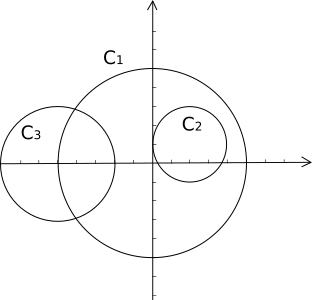
\includegraphics[height=5cm]{circles.png}
        \caption{Overlapping circles $C_1$, $C_2$ and $C_3$.}
        \label{fig:circles}
    \end{figure}

    % \Question{We can make this code interactive by using the {\tt input()} function. Use the {\tt input()} function to ask the user the age of their cat.}
    % \Question{(*) Can you make a game where a user tries to predict the roll of a dice? Let them know if their guess was too low or too high, and how close it was.
    
    % \textbf{Hint:} Recall you replicated dice throws in Week 1 - Ex.\ref{Ex:Import_Modules}.}
\end{Exercise}

\subsection*{Checklist}
\begin{itemize}
    \item Meet your TA - they will be mentoring you throughout the course, and will be there to answer questions and provide feedback along the way.
	\item Check that you understand the basics: variables, different types of variables (integers, floats, complex, Booleans, strings), the different built-in operators, and how these work with both numbers and strings.
	\item Practice with using the IDLE shell as a useful calculator with access to some powerful abilities provided in ``modules''.
    \item Check you are familiar with variable naming styles and conventions.
    \item Know how to make and run a python file script.
	\item Learn about conditional statements, and how these are used to control the flow of the program.
\end{itemize}

\subsection*{Additional resource}
\begin{itemize}
    \item Check the `Additional Resources' folder on Blackboard, where you will find video tutorials on how to download and install Python 3 and using IDLE. Keep an eye on this folder as it'll be regularly updated with tutorials and guides.
	\item There are many online tutorials for Python 3, so if you're wondering what more you can do, please do search online or ask your TAs for pointers.
\end{itemize}

\end{document}